\chapter{Konzolová časť aplikácie na správu mikrotikov}
V tejto kapitole si popíšeme fungovanie naprogramovanej aplikácie. Celkovo je konzolová časť aplikácie napísaná za pomoci knižnice tikapy popísanej v kapitole \ref{sec:tikapy}. Kapitola bude rozdelená do niekoľkých častí:\begin{itemize}
\item časť 1: popis naprogramovanej časti pre vyhľadávanie mikrotikov, pripojenie sa na mikrotik cez python pomocou protokolov telnet, SSH, mactelnet a napojenie na metódy
\item časť 2: Popis infraštruktúry backendu - zložky, ich vysvetlenie, zoznam súborov na konfiguráciu mikrotku, vysvetenie rozdelenia, vysvetlenie tried, metód daných tried a volanie funkcií
\item časť 3 - prtidanie tabuliek jednotlivých tried a ich metód v každej zložke, krátka sumarizácia, ich niektoré vybrané UML diagramy, ostatné budú zahrnuté v prílohe
\end{itemize}
\section{Popis naprogramovanej časti prihlasovania na mikrotik}
\label{sec:popis1}
V tejto časti si zobrazíme rozbor časti prihlasovania na mikrotik a základné funnkcie. Toto je riadené v rámci projektu nazvaného \textit{diplomkap3} v ktorom je súbor \textit{loginManager.py}. V rámci login managera tu nachádzame ďalšie súbory, ktoré sú zobrazené na obrázku \ref{fig:filesLogin}. 
\begin{figure}[H]
\centering
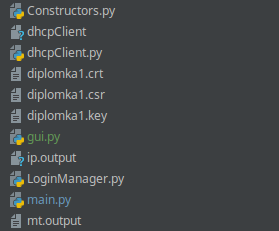
\includegraphics[scale=0.6]{../text/loginFiles.png}
\caption{Zoznam základných konfiguračných súborov}
\label{fig:filesLogin}
\end{figure} 
\subsection{Súbor centralControl}
\label{sec:central}
V súbore centrolControl sa popisuje spôsob hromadnej obsluhy mikrotikov na základe protokolu mactelnet. Pozostáva z metód:
\begin{itemize}
\item \textit{konštruktor} - pozostáva zužívateľských mien a hesiel, heslá v premennej credentials sú uložené ako slovník v podobe IP adresa: heslo
\item \textit{listMikrotikDevices()} - metóda vráti zoznam MAC a IP adries nájdených mikrotikov, uloží ich do súboru, a finálny výstup predstavuje list MAC adries
\item \textit{addCredentials()} - metóda pridíva heslo k užívateľskému účtu do slovníku, štandardnéužívateľské meno sa používa admin, ale tiež sa môže použiť aj iné užívateľské meno pri volaní metódy
\item \textit{loginSSH()}- metóda je použitá na hromadné prihlásenie pomoocu protokolu SSH na mikrotiky, používa sa tu pritom knižnica pexpect a jej subkižnica pxssh, jej vstupné parametre sp IP adresa serveru, užívateľské meno a heslo 
\end{itemize}
\begin{sexylisting}{Konštruktor súboru}
 def __init__(self, login):
        self.username = login
        self.credentials = {
            "192.168.1.1": "admin",
            "192.168.2.1": ""
        }
\end{sexylisting}
\begin{sexylisting}{Meóda zobrazenia mikrotikov}
 def listMikrotikDevices(self):
   deviceList = []
   loadAddress = False
   os.system("mactelnet -l -t 20 2>&1 > mt.output")
    with open( "mt.output", "r" ) as file:
     for line in file:
      if loadAddress:
         address = line.split( )[0]
         deviceList.append( address )
      else:
         header = line.split( )
         if len( header ) > 1:
            if "IP" in header[0]:
              loadAddress = True
         for i in deviceList:
           print(i)
  return deviceList
\end{sexylisting}
\begin{sexylisting}{Metóda pridania užívateľských mien a hesiel}
 def addCredentials(self, login="admin"):
   server_list = self.listMikrotikDevices()
   print( server_list )
   for server in server_list:
   try:
    password = self.credentials[server]
    except KeyError:
    password = input( "Please eneter the 
    password for " + server + ":" )
    self.credentials[server] = password
    return server_list
\end{sexylisting}
\begin{sexylisting}{Metóda hromadného prihlásenia pomocou protokolu SSH}
def loginSSH(self, server,login, password):
 from pexpect import pxssh, spawn, expect
 import getpass
 for server in self.credentials:
 try:
  connect = pxssh.pxssh( )
  server = self.credentials
  login = 'admin'
  password = self.credentials[server]
  port = 22
  connect.login( server, login, password )
  commands = pxssh.spawn( )
  time.sleep( 10 )
 except pxssh.ExceptionPxssh as e:
  print( "Error" )
  print( str( e ) )
\end{sexylisting}
\subsection{Súbor Constructors}
Súbor predstavuje zoznam konštruktorov pre konkrétne naprogramované API moduly pomocou knižnice tikapy. V úvode konštruktoru sú popísané importy jednotlivých modulov a submodulov pre konfiguráciu mikrotiku za pomoci API. \\
Následne je vytvorená trieda Mikrotik, ktorá zahŕňa všetky konštruktory spoločne s ich vstupnými parametrami, ktoré sú adresa,užívateľské meno a heslo. 
\begin{figure}[H]
\centering
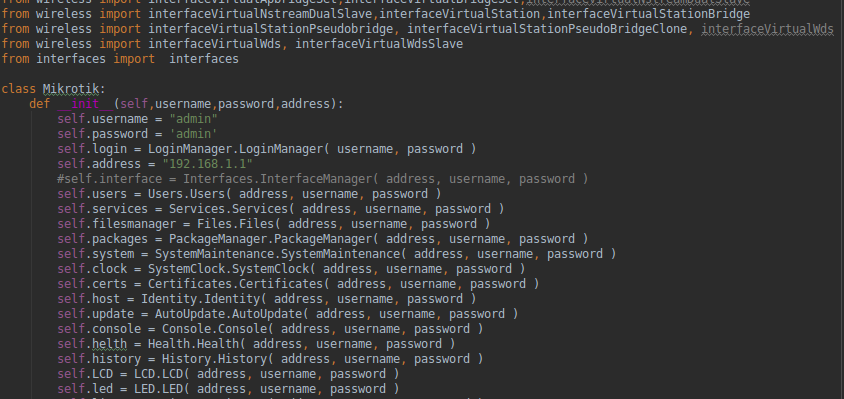
\includegraphics[scale=0.5]{../text/constructors.png}
\caption{Ukážka konštruktorov projektu}
\label{fig:constructors}
\end{figure} 
\subsection{Súbor dhcpClient}
V tomto súbore sa nachádza základná konfigurácia mikrotiku po pripojení naň. Obsahuje triedu basicConfig, ktorá pozostáva z dvoch metód.\\
V konštruktore sa nastaví rozhranie, na ktorom sa má adresa nastaviť, IP adresa/subnet a MAC adresa na pripojenie na mikrotik pomocu protokolu mactelnet.\\
\begin{sexylisting}{Trieda basicConfig}
class basicCOnfig:
    def __init__(self,interface,mac,ip):
        self.interface = interface
        self.mac = mac
        self.ip = ip
\end{sexylisting}
Prvá metóda \textit{dhcp()}, ktorej vstupné parametre sú užívateľské meno a heslo. Pozostáva z prihlásenia na mikrotik, a nastavenia Dynamic Host Client Protocol (DHCP) klienta na rozhraní, ktoré sa definuje pri volaní objektu v rámci konštruktoru.\\
\begin{sexylisting}{Metóda dhcp}
 def dhcp(self,username,password):
        child =pexpect.spawn('mactelnet '+self.mac)
        child.expect('Username:')
        child.sendline(username)
        child.expect('Password:')
        child.sendline(password)
        child.sendline('\r')
        try:
            child.expect('> ')
            child.sendline('ip dhcp-client add 
            interface='+self.interface+"\r")
            child.expect('> ')
            child.close()
        except:
            print("error")
            child.close()
        time.sleep(1)
\end{sexylisting}
Druhá metóda \textit{setAddress()}, ktorá bere ako vstupné parametre užívateľské meno a heslo nastaví statickú IP adresu na rozhraní definovanom v rámci konštruktoru.
\begin{sexylisting}{Metóda setAddress}
    def setAddress(self,username,password):
        child = pexpect.spawn( 'mactelnet '+ 
        self.mac )
        child.expect( 'Username:' )
        child.sendline( username )
        child.expect( 'Password:' )
        child.sendline( password )
        child.sendline( '\r' )
        try:
            child.expect( '> ' )
            child.sendline( 'ip address add address='
            +self.ip + " interface="
            +self.interface+"\r" )
            child.expect( '> ' )
            child.close()
        except:
            print( "error" )
            child.close()
        time.sleep( 1 )
\end{sexylisting}
\subsection{Súbor LoginManager}
Súbor LoginManager pozostáva z niekoľkých metód, tieto metódy majú podobnú štruktúru ako súbor centralConrol popisujúci v kapitole\ref{sec:central}.\\
Ako prvá popísaná časť je konštruktor, ktorý prijíma vstupné parametre užívateľské meno a heslo.\\
\begin{sexylisting}{Konštruktor súboru}
    def __init__(self, login,password):
        self.username = login
        self.pwd = password
\end{sexylisting}
Druhá metóda je metóda \textit{loginTelnet()},v rámci tejto metódy sa rieši prihlásenie na mikrotik pomocou protokolu telnet za použitia knižnice telnetlib. Vo vstupe metódy sa definuje premenná \textit{server_list}. Táto premenná je naplnená IP adresami mikrotikov v rámci súboru centralControl.\\
\begin{sexylisting}{Metóda loginTelnet}
    def loginTelnet(self, password, login="admin"):
        import telnetlib
        central = centralControl(login, password)
        server_list = central.listMikrotikDevices()
        print(server_list)
        for server in server_list:
            try:
                telnetcon = telnetlib.Telnet
                ( host=server, port=23 )
                telnetcon.read_until( b"Login: " )
                telnetcon.write( login.encode( )
                 + "\n" )
                telnetcon.read_until( b"Password: " )
                telnetcon.write( password.encode( )
                 + b"\n" )
                time.sleep( 10 )
                telnetcon.close( )
            except:
                print( "Cannot connect to 
                router via telnet" )
\end{sexylisting}
Ďalej sa tu nachádza metóda loginSSH(), táto metóda pracujúca podobne ako metoda loginTelnet() pracuje na základe protokolu SSH, na vstupe má server IP adresu, užívateľské meno  a heslo. \\
\begin{sexylisting}{Metóda loginSSH}
    def loginSSH(self, server,login, password):
        from pexpect import pxssh, spawn, expect
        import getpass
        try:
            connect = pxssh.pxssh( )
            server = '172.16.49.2'
            login = 'admin'
            password = 'admin'
            port = 22
            connect.login( server, login, 
            password )
            commands = pxssh.spawn( )
            time.sleep( 10 )
        except pxssh.ExceptionPxssh as e:
            print( "Error" )
            print( str( e ) )
\end{sexylisting}
Ďalšou metódou je metóda na vylistovanie všetkýchmikrotikov, táto metóda je bez vstupného parametru. Ako výstup je súbor mikrtik.output naplnený MAC adresami mikrotikov. 
\\
\begin{sexylisting}{Metóda listMikrotikDevices}
    def listMikrotikDevices(self):
        deviceList = []
        loadMacAddress = False
        os.system("mactelnet -l -t 20 
        2>&1 > mt.output")
        with open( "mt.output", "r" ) 
        as file:
            for line in file:
                if loadMacAddress:
                   macAddress = line.split( )[1]
                   deviceList.append( macAddress )
                else:
                    header = line.split( )
                    if len( header ) > 1:
                        if "IP" in header[0] 
                        and "MAC-Address" 
                        in header[1]:
                            loadMacAddress = True
        return deviceList
\end{sexylisting}
Poslednou metódou je metóda \textit{mactelnetLoginToSingleDevice()}, vďaka ktorej sa pripája pomocou protokolu mactelnet na jedno mikrotik zariadenie pomocou macadresy získanej z výstupu metódy \textit{listMikrotikDevices()} \textit{mikrotik.output}.
\begin{sexylisting}{Metóda mactelnetLoginToSingleDevice}
    def mactelnetLoginToSingleDevice(self, username, 
    password, address=None):
        deviceList = self.listMikrotikDevices()
        print( deviceList )
        if address:
            print('mactelnet {} -u {} -p {}'.format
            ( address, username, password ))
            os.system( 'mactelnet {} -u {} -p {}'.format
            ( address, username, password ) )
        elif deviceList:
            print( 'mactelnet {} -u {} -p {}'.format
            ( deviceList[0], username, password ) )
            os.system( 'mactelnet {} -u {} -p {}'.format
            ( deviceList[0], username, password ) )
        else:
            print("No device was found")
\end{sexylisting}
\section{Rozbor hlavnej časti backendu}
V rámci hlavnej konfiguračnej časti diplomovej práce, pre konfiguráciu backendu mikrotiku za pomoci porgramovacieho jazyka python som projekt rozdelil do niekoľkých častí:\begin{itemize}
\item \textbf{bridge} - táto časť obsahuje prvky konfiguácie, pridania, odstránenia, zapnutia, vypnutia možnosti bridgu na mikrotiku, konfigurácia existujúceho bridgu, zobrazenie zoznamu bridgov
\item  \textbf{capsman} - táto časť obsahuje konfiguráciu hromadnej obsluhy mikrotik úrístupových bodov a WiFi, profily, bezpečnosť, konfiguácie, povolené rýchlosti, zobrazenie zoznamu pripojených prvkov a ďalšie funkcie
\item \textbf{certs} - obsahuje certifikáty na pripojenie sa na mikrotik pomocou protokolu api-ssl
\item \textbf{Dude} - obsahuje popis konfigurácie ako nastaviť nástroj Dude klienta, ako nakonfigurovať Dude na vzdialený monitoring na Dude serveri, taktiež Dude server, a ďalšie možnosti
\item \textbf{exportToHtml} - časť predstavuje generovanie súboru na analýzu v podobe webovej stránky
\item \textbf{interfaces} - časť predstavuje konfiguráciu rozhraní na mikrotiku, tieto časti sú tiež popísané aj v iných zložkách ako napr. bridge. 4asť popisuje pridanie, odstránenie, zapnutie, vypnutie, konfiguráciu existujúcich rozhraní.
\item \textbf{IPv4} - rozsiahla časť, obsahuje konfiguráciu IP adries, firewallu, monitoringu, smerovania a ďalších nástrojov spadajúcich pod IP zložku na mikrotiku.
\item \textbf{IPv6} - pre zložku IPv6 platí to isté čo pre zložku IPv4, ale platí pre konfiguráciu na základe IPv6 adresného rozsahu
\item \textbf{KVM} - sekcia bude popisovať možnosti virtualizácie mikrotiku.
\item \textbf{log} - sekcia bude popisovať analýzu a konfiguráciu logu zariadenia
\item \textbf{makeSupportFile} - seckia bude popisovať vytvorenie súboru potrebného pre analýzu na mikrotik podpore
\item \textbf{mesh} - sekcia popisuje konfiguráciu tzv. mesh technológie, technológii podobne ako  v rámci časti bridge
\item \textbf{MPLS} - sekcia bude popisovať možnosti konfiurácie Multi Protocol Label Switching (MPLS), jej pridanie, odstránenie ,zapnutie, vypnutie, modifikácie a ďalšie funkcie.
\item \textbf{PPP} - sekcia bude popisovať konfiguráciu Point to Point Protocol (PPP) a ďalších možností Virtual Private Network (VPN) konfigurácie.
\item \textbf{Queues} - sekcia budep popisovať konfiguráciu sieťových front, možnosti front, typy front a ďalšie funkcie
\item \textbf{Radius} - sekcia bude popisovať nastavenie funkcie Radius - autentizačnej služby užívateľov , jeho modifikáciu, konfiguráciu a ďalšie funkcie.
\item \textbf{Routing} - sekcia bude popisovať možnosti dynamického smerovania, statické smerovanie bude popísané v rámci časti IPv4, dynamické smerovacie protokoly, ich konfigurácie, a ďalšie možnosti. 
\item \textbf{Switch} - sekcia bude popisovať konfiguráciu prepínača, niektoré mikrotiky sú typu SwitchOS a sú štandardne prepínač. Kofiguuráciu portov, trunkov, a ďalších funkcií. 
\item \textbf{System} - sekcia bude popisovať časť konfigurácie systémových nástrojov, ich funkcií a konfigurácie, a ďalších funkcií.
\item \textbf{Tools} - sekcia bude popisovať konfiguráciu mikrotik nástroj, a však nie všetky bolo možné odsimulovať v rámci konzolvej časti aplikácie, ich konfiguráciu, spustenie, riadenie a ďalšie funkcie. 
\item \textbf{Wireless} - sekcia bude obsahovať konfiguráciu bezdrátového rozhrania, moduly, módy, konfiguráciu, nastavenie, a ďalšie funkcie
\item \textbf{konfiguračné súbory mimo zložiek} - sekcia popísaná v kapitole  \ref{sec:popis1}, popisuje súbory na základnú konfiuráciu mikrotiku, nastavenie základnej konfigurácie.
\end{itemize}
Ukážka súborovej štruktúry je zobrazená na obrázku \ref{fig:structure}:
\begin{figure}[H]
\centering
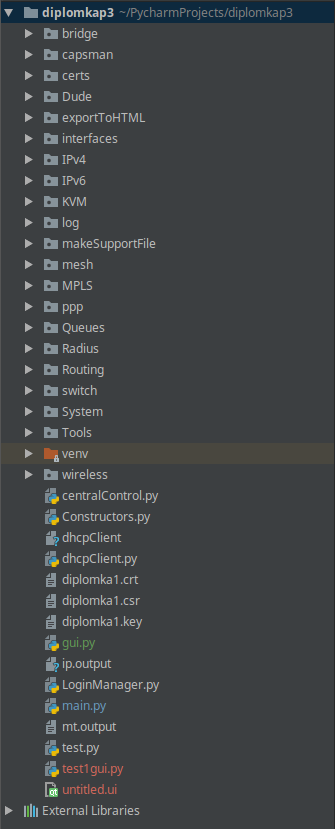
\includegraphics[scale=0.4]{../text/struktura.png}
\caption{Štruktúra projektu konzolovej časti projektu}
\label{fig:structure}
\end{figure} 
\chapter{Hlavná časť backendu}
Cieľom kapitoly je detailný popis backend časti aplikácie na správu mikrotikov. V jendotlivých podkapitolách bude popísaná každá zložka projektu diplomkap3.
\section{Zložka bridge}
Cieľom tejto zložky je konfigurácia bridgu na mikrotiku. Pozostáva z:\begin{itemize}
\item Managementu bridgu, portov, bezpečnosti, pripojených zariadení
\item Pridanie, odtsránenie, zapnutie, vypnutie a komentár položiek
\item Modifikácia existujúcich položiek
\end{itemize}
\begin{figure}[H]
\centering
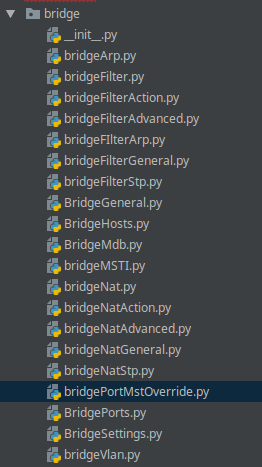
\includegraphics[scale=0.57]{../text/bridgeList.png}
\caption{Zoznam súborov zložky bridge}
\label{fig:bridge2}
\end{figure} 
Niektoré pasáže sa dajú modifikovať pomocou mena položky, niektoré pomocou poradia položky. Zoznam súborov  zložky nájdeme na obrázku \ref{fig:bridge2} a v kapitole\ref{sec:bridgechap}. 
\subsection{Popis tried zložky}
\label{sec:bridgechap}
Zložka obsahuje triedy:
\begin{itemize}
\item \textbf{bridgeArp} - trieda nastavuje funkcionalitu ARP v rámci bridgu
\item \textbf{bridgeFilter} - trieda nastavuje funkcionalitu fitrovania provozu (firewall)
\item \textbf{bridgeFilterAction} - trieda nastavuje akcie filtrovania provozu
\item \textbf{bridgeFilterAdvanced} - trieda nastavuje pokročilé filtrovanie
\item \textbf{bridgeFilterGeneral} - trieda nastavuje genrálne nastavenie filtrovania provozu
\item \textbf{bridgeHosts} - trieda ošetruje zoznam pripojených zariadení na bridge
\item \textbf{bridgeMdb} - trieda ošetruje nastavenie portov pripojených zariadení
\item \textbf{bridgeMSTI} - trieda nastavuje MST modul bridgu
\item \textbf{bridgeNAT} - trieda oošetruje nastaveneie NAT na bridgi
\item \textbf{bridgeNATAction} - trieda ošetruje nastavenie akcií NAT
\item \textbf{bridgeNatAdvanced} - trieda ošetruje pokročilé nastavenie NAT
\item \textbf{bridgeNatGeneral} - trieda ošetruje genrálne nastavenie NAT na bridgi
\item \textbf{bridgeNatStp} - trieda ošetruje nastavenie STP
\item \textbf{bridgePortMstOverride} - trieda ošetruje nastavenie nanútenia MST
\item \textbf{BridgePorts} - trieda ošetruje nastavenie portov bridgu
\item \textbf{BridgeSettings} - trieda ošetruje globálne nastavenie  bridgu  
\item \textbf{BridgeVlan} - trieda ošetruje globálne nastavenie VLAN
\subsection{Vybraný analyzovaný súbor}
Ako ukážku je vybratý súbor bridgeArp s popisom metód v tabuľke \ref{tab:bridge1}.
\begin{table}[H]
\resizebox{\textwidth}{!}{%
\begin{tabular}{|c|c|c|c|}
\hline
Názov metódy & Vstup & Výstup & Vysvetlenie metódy \\ \hline
setArpOpcode & \begin{tabular}[c]{@{}c@{}}číslo bridgu,\\ operátor\end{tabular} & slovník & \begin{tabular}[c]{@{}c@{}}Metóda nastaví operačný mód ARP\\ - arp-nak, darp-error,...\end{tabular} \\ \hline
setArpHadrwareType & \begin{tabular}[c]{@{}c@{}}číslo bridgu,\\ operátor\end{tabular} & slovník & Metóda nastaví typ hardvéru (číslený kód) \\ \hline
setArpPacketType & \begin{tabular}[c]{@{}c@{}}číslo bridgu,\\ typ paketu(číselné označenie)\end{tabular} & slovník & Metóda nastaví typpaketov \\ \hline
setArpSrcAddrr & \begin{tabular}[c]{@{}c@{}}číslo bridgu,\\ zdrojová adresa\end{tabular} & slovník & Metóda nastaví zdrojovú adresu bridgu \\ \hline
setArpSrcmAcAdress & \begin{tabular}[c]{@{}c@{}}číslo bridgu,\\ zdrojová MAC adresa,\\ maska MAC adresy\end{tabular} & slovník & Metóda nastaví zdrojovú MAC adresu bridgu \\ \hline
setArpDstmAcAdress & \begin{tabular}[c]{@{}c@{}}číslo bridgu,\\ cieľová MAC adresa\end{tabular} & slovník & Metóda nastaví cieľovú MAC adresu bridgu. \\ \hline
setArpGratitinuous & \begin{tabular}[c]{@{}c@{}}číslo bridgu, \\ typ arp(štandardne none)\end{tabular} & slovník & Metóda nastaví typ ARP \\ \hline
\end{tabular}%
}
\caption{Tabuľka zoznamu metód triedy bridgeArp}
\label{tab:bridge1}
\end{table}
\end{itemize}
\begin{figure}[H]
\centering
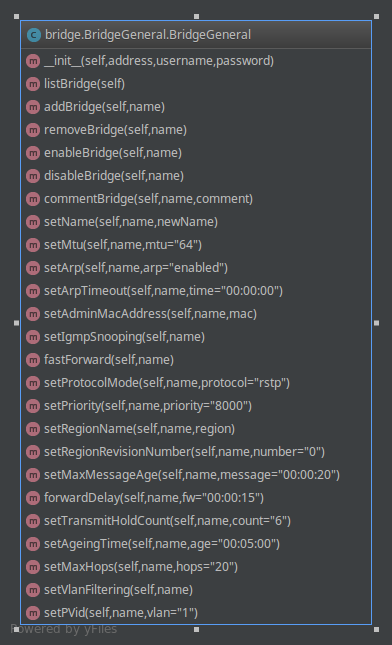
\includegraphics[scale=0.48]{../text/bridge.png}
\caption{UML diagram vybraného súboru bridgeArp}
\label{fig:bridge}
\end{figure}
\section{Zložka capsman}
\label{sec:capsmanchap}
Súčasťou zložky capsman sú súbory na centrálne nastevenie WiFi pomocou mikrotik funkcionality capsman. Capsman dovoľuje nastaviť a centrálne riadiť prístupové body na centrálnom smerovači.
Zložka pozostáva z:\begin{itemize}
\item Správu nakonfigurovaných položiek
\item Pridávanie, odstránenie, zapnutie, vypnutie a koment položiek
\item Modifikácia nakonfigurovaných položiek
\item Správa pripojených zariadení
\end{itemize}
\\Zoznam súborov nájdeme na obrázku \ref{fig:capsman}. 
\begin{figure}[H]
\centering
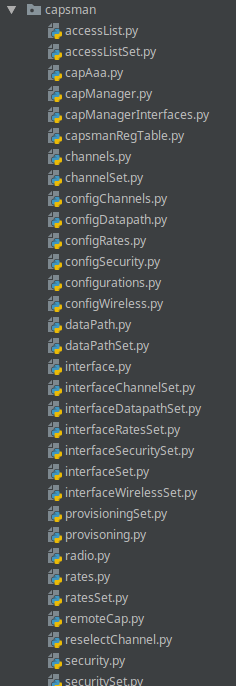
\includegraphics[scale=0.6]{../text/capsman.png}
\caption{Zoznam súborov zložky capsman}
\label{fig:capsman}
\end{figure}
\subsection{Popis tried zložky}
Zložka obsahuje:\begin{itemize}
\item \textbf{accessList} - trieda ošetruje nastavenie prístupých listov (access listov)
\item \textbf{accessListSet}- trieda ošetruje nastavenie už vytvorených access listov
\item \textbf{capAaa} - trieda ošetruje nastavenie autorizačného protokolu  AAA
\item \textbf{capManager} - trieda ošetruje nastavenie capsman managera
\item \textbf{capManagerInterfaces}- trieda ošetruje nastavenie capsman rozhraní
\item \textbf{capsmanRegTable} - trieda obsahuje zoznam zaregistrovaných zariadení  a ich publikácia (provisioning)
\item \textbf{channel} - trieda ošetruje nastavenie kanálov v rámci WIFi pre centrálne riadenie capsmanom
\item \textbf{channelSet} - trieda ošetruje nastavenie už existujúcich profilov kanálov 
\item \textbf{configChannels} - trieda ošetruje nastavenie kanálov v rámci globálnej konfigurácie WiFi v rámci  capsman
\item \textbf{configDatapath} - trieda očetruje nastavenie dátových ciest (datapath) v rámci globálneho konfiguračného súboru 
\item \textbf{configRates} - trieda ošetruje nastavenie povolených prenosových rýchlostí 
\item \textbf{configSecurity} - trieda ošetruje nastavenie bezpečnosti
\item \textbf{configurations} - trieda ošetruje management, pridávanie, odstránenie, povolenie, zakázanie a komentovanie konfiguračných súborov
\item \textbf{configWireless} - trieda ošetruje nastavenie Wireless rozhrania
\item \textbf{dataPath} - trieda ošetruje management dataPath, pridávanie, odstránenie, povolenie ,zakázanie a komentovanie
\item \textbf{dataPathSet} - trieda ošetruje nastavenie už existujúcich dátových ciest
\item \textbf{interface} - trieda ošetruje management rozhraní riadených capsmanom
\item \textbf{interfaceChannelSet} - trieda ošetruje nastavenie kanálov v rámci rozhrania
\item  \textbf{interfaceDatpathSet} - trieda ošetruje nastavenie dátových ciest v rámci konfigurácie rozhrania capsman
\item \textbf{interfaceRatesSet} - trieda ošetruje nastavenie povolených rýchlostí v rámci konfigurácie rozhrania capsmanom
\item  \textbf{interfaceSecuritySet} - trieda ošetruje nastavenie bezpečnosti v rámci capsman rozhrania
\item \textbf{interfaceSet} - trieda ošetruje základnú konfiguráciu rozhrania 
\item \textbf{interfaceWirelessSet} - trieda ošetruje nastavenie WiFi profilu
\item \textbf{provisioningSet} - trieda ošetruje možnosti publikácie konfigurácie - statické, dynamické
\item \textbf{provisioning} - trieda ošetruje management publikácie konfigurácií
\item \textbf{radio} -  trieda ošetruje nastavenie publikácie pripojných prístupových bodov
\item \textbf{rates} - trieda ošetruje management povolených prenosových rýchlostí
\item \textbf{ratesSet} - trieda ošetruje nastavenie prenosových rýchlostí
\item \textbf{remoteCap} - trieda ošetruje správu pripojených prístupových bodov - upgrade, publikáciu
\item \textbf{reselectChannnels} - trieda ošetruje výber druhého kanálu prístupového bodu
\item \textbf{secuirity} - trieda ošetruje management bezpečnostných profilov - pridávanie, odstránenie, povolenie ,zakázanie a komentovanie
\item \textbf{securitySet} - trieda ošetruje nastavenie bezpečnosti už existujúcich profilov
\end{itemize}
\subsection{Vybraný analyzovaný súbor}
Pre analýzu jedného súboru zo zložky je vybratý súbor \textit{configRates.py}. Jeho UML diagram je zobrazený na obrázku \ref{fig:capsman1} a zoznam jeho metód je popísaný v tabuľke \ref{tab:rates}.
\begin{figure}[H]
\centering
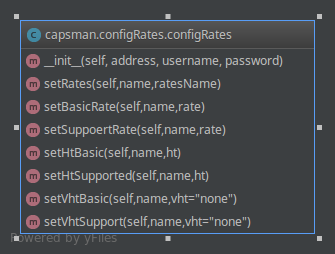
\includegraphics[scale=0.6]{../text/configRates.png}
\caption{UML diagram triedy configRates}
\label{fig:capsman1}
\end{figure}
\begin{table}[H]
\resizebox{\textwidth}{!}{%
\begin{tabular}{|c|c|c|c|}
\hline
Názov metódy & Vstup & Výstup & Vysvetlenie metódy \\ \hline
setRates & \begin{tabular}[c]{@{}c@{}}názov profilu,\\ nové meno\end{tabular} & slovník & Metóda premenuje profil \\ \hline
setBasicRate & \begin{tabular}[c]{@{}c@{}}názov profilu,\\ základné prenosové rýchlosti\end{tabular} & slovník & Metóda nastaví prenosovú rýchlosť. \\ \hline
setSuppoertRate & \begin{tabular}[c]{@{}c@{}}názov profilu,\\ podporované prenosové rýchlosti\end{tabular} & slovník & Metóda nastaví posporované prenosové rýchlosti. \\ \hline
setHtBasic & \begin{tabular}[c]{@{}c@{}}názov profilu,\\ základný prenosový kanál(y)\end{tabular} & slovník & Metóda nastaví prenosový kanál. \\ \hline
setHtSupported & \begin{tabular}[c]{@{}c@{}}názov profilu,\\ podporované prenosové kanály\end{tabular} & slovník & Metóda nastaví podporované prenosové kanály. \\ \hline
setVhtBasic & \begin{tabular}[c]{@{}c@{}}názov profilu,\\ základné virtuálne kanály\end{tabular} & slovník & Metóda nastaví prenosový virtuálny kanál. \\ \hline
setVhtSupport & \begin{tabular}[c]{@{}c@{}}názov profilu,\\ podporované prenosové virtuálne kanály\end{tabular} & slovník & Metóda nastaví podporované prenosové kanály. \\ \hline
\end{tabular}%
}
\caption{Popis triedy configRates}
\label{tab:rates}
\end{table}
\section{Zložka Dude}
Popisovaná zložka je obsah tried,ktoré nastavujú Dude monitorovací nástroj. Plnia rovnakú funkciu ako je to popísané v kapitolách \ref{sec:bridgechap} a \ref{sec:capsmanchap}. Na obrázku \ref{fig:dude} vidíme zoznam súborov. 
\subsection{Popis tried zložky}
Súčasťou zložky je nastavenie nástroja Dude na centrálny monitoring mikrotikov. Obsahuje súbory:\begin{itemize}
\item \textbf{Devices} - trieda ošetruje nastavenie monitorovaných zariadení
\item \textbf{Notifications} - trieda ošetruje nastavenie upozornení
\item \textbf{Probes} - trieda ošetruje nastavenie tetsovaní spojenia
\item \textbf{RosInfo} - trieda ošetruje výpis informácií ohľadom hardvéru a operačného systému routerOS
\item \textbf{Services} - trieda ošetruje nastavenie služieb
\item \textbf{Settings} - trieda ošetruje zapnutie a vypnutie Dude nástroju
\item \textbf{ostatné knižnice} - osotatné knižnice API nepodporuje
\end{itemize}
\begin{figure}[H]
\centering
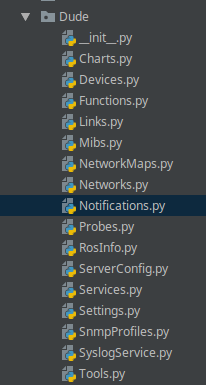
\includegraphics[scale=0.6]{../text/dude.png}
\caption{Zoznam súborov adresáru Dude}
\label{fig:dude}
\end{figure}
\subsection{Analýza vybraného súboru}
Vybraný analyzovaný súbor \textit{Devices.py} a jeho analýza je popísaná v rámci jeho UML diagramu na obrázku \ref{fig:dudedev} a zoznam metód je popísaný v tabuľke \ref{tab:devices}.
\begin{figure}[H]
\centering
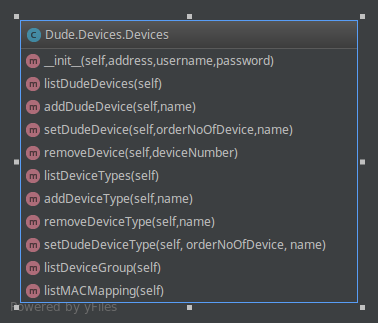
\includegraphics[scale=0.6]{../text/DudeDev.png}
\caption{UML diagram knižnice Devices}
\label{fig:dudedev}
\end{figure}
\begin{table}[H]
\resizebox{\textwidth}{!}{%
\begin{tabular}{cccc}
\hline
\multicolumn{1}{|c|}{Názov metódy} & \multicolumn{1}{c|}{Vstup} & \multicolumn{1}{c|}{Výstup} & \multicolumn{1}{c|}{Vysvetlenie metódy} \\ \hline
\multicolumn{1}{|c|}{listDudeDevices} & \multicolumn{1}{c|}{žiadny} & \multicolumn{1}{c|}{slovník} & \multicolumn{1}{c|}{Metóda vypíše zoznam Dude zariadení.} \\ \hline
\multicolumn{1}{|c|}{addDudeDevice} & \multicolumn{1}{c|}{názov zariadenia} & \multicolumn{1}{c|}{slovník} & \multicolumn{1}{c|}{Metóda pridá nové zariadenie} \\ \hline
\multicolumn{1}{|c|}{setDudeDevice} & \multicolumn{1}{c|}{\begin{tabular}[c]{@{}c@{}}číslo zariadenia,\\ meno zariadenia\end{tabular}} & \multicolumn{1}{c|}{slovník} & \multicolumn{1}{c|}{Metóda premenuje zariadenie.} \\ \hline
\multicolumn{1}{|c|}{removeDevice} & \multicolumn{1}{c|}{číslo zariadenia} & \multicolumn{1}{c|}{slovník} & \multicolumn{1}{c|}{Metóda zmaže zariadenie.} \\ \hline
\multicolumn{1}{|c|}{listDeviceTypes} & \multicolumn{1}{c|}{žiadny} & \multicolumn{1}{c|}{slovník} & \multicolumn{1}{c|}{Metóda zobrazí typy zariadení.} \\ \hline
\multicolumn{1}{|c|}{addDeviceType} & \multicolumn{1}{c|}{názov zariadenia} & \multicolumn{1}{c|}{slovník} & \multicolumn{1}{c|}{Metóda pridá nové zariadenie.} \\ \hline
\multicolumn{1}{|c|}{removeDeviceType} & \multicolumn{1}{c|}{názov profilu} & \multicolumn{1}{c|}{slovník} & \multicolumn{1}{c|}{Metóda zmaže typ zariadenia.} \\ \hline
\multicolumn{1}{l}{} & \multicolumn{1}{l}{} & \multicolumn{1}{l}{} & \multicolumn{1}{l}{} \\
\multicolumn{1}{l}{} & \multicolumn{1}{l}{} & \multicolumn{1}{l}{} & \multicolumn{1}{l}{} \\
\multicolumn{1}{l}{} & \multicolumn{1}{l}{} & \multicolumn{1}{l}{} & \multicolumn{1}{l}{}
\end{tabular}%
}
\caption{Tabuľka metód triedy Devices}
\label{tab:devices}
\end{table}
\section{Zložka Interfaces}
Popisovaná zložka je obsah tried,ktoré nastavujú rozhrania na mikrotiku. Medzi tieto rozhrania patria nastavenie VPN, ethernet, WiFi rozhraní a ďalších rozhraní. Plnia rovnakú funkciu ako je to popísané v kapitolách \ref{sec:bridgechap} a \ref{sec:capsmanchap} a ďalších kapitolách. Na obrázku \ref{fig:iface} vidíme zoznam súborov.
\subsection{Popis tried zložky}
Súčasťou zložky je nastavenie rohraní na mikrotiku. Patria sem triedy:
\begin{itemize}
\item \textbf{bonding} - trieda ošetruje nastavenie bonding rozhrania, rozhrania na nastevnie failover technológie súčasne s ďalšimi dvomi triedami na nastavenie bonding - \textbf{bondingGeneralSet} a \textbf{bondingSet} 
\item \textbf{detectInternet} - trieda detekuje internet na vybranom rozhraní
\item \textbf{eoipTunel} - trieda nastaví ethernet over IP rozhranie,spoločne s triedami \textbf{eoipSetGeneral} a \textbf{eoipSetLoopProtection}
\item \textbf{ethernet} - trieda nastaví ethernet rozhrania spoločne s triedami \textbf{ethernetSet}, \textbf{ethernetSetGeneral} a \textbf{ethernetLoopProtectionSet}
\item \textbf{greTunnel} - trieda nastaví rozhranie typu tunel GRE spoločne s triedou \textbf{greTunnelSet}
\item \textbf{interfaceList} - trieda nastaví listrozhraní spoločne s triedou \textbf{interfaceListSet}
\item \textbf{interfaces} - trieda zobrazí  a nastaví všetky rozhrania na mikrotiku
\item \textbf{interfaces} - trieda nastaví Long Term Evolution (LTE) rozhranie
\item \textbf{ipTunnel} - trieda nastaví IP tunel spoločne s triedou \textbf{ipTunnelSet}
\item \textbf{lists} - trieda nastaví listy rozhraní spoločne s triedou \textbf{listsSet}
\item \textbf{lteApn} - trieda nastaví prístupové LTE body spoločne s triedou \textbf{lteApnSet}
\item \textbf{vlan} - trieda nastaví VLAN spoločne s triedami \textbf{vlanLoopProtection} a \textbf{vlanSetGeneral}
\item \textbf{vrrp} - trieda nastaví zálohovací mechanizmus  Virtual Router Redoundency Protocol (VRRP) spoločne s triedami \textbf{vrrpGeneralSet, vrrpScriptSet a vrrpSetVrrp}
\end{itemize}
\begin{figure}[H]
\centering
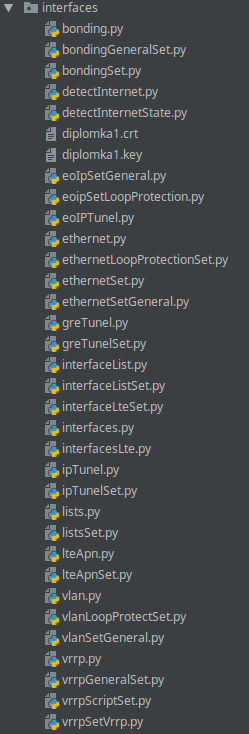
\includegraphics[scale=0.6]{../text/interfaces.png}
\caption{Zoznam súborov adresáru Interfaces}
\label{fig:iface}
\end{figure}
\subsection{Analýza vybraného súboru}
Vybraný súbor \textit{greTunnelSet.py} a jeho nastavenie je zobrazené v UML diagrame triedy na obrázku \ref{fig:gre} a popis tried je zanalyzovaný v tabuľke \ref{tab:greTunel}.
\begin{figure}[H]
\centering
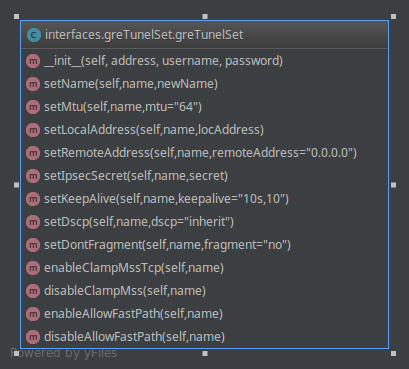
\includegraphics[scale=0.6]{../text/gre.png}
\caption{UML diagram greTunnelSet triedy}
\label{fig:gre}
\end{figure}
\begin{table}[H]
\resizebox{\textwidth}{!}{%
\begin{tabular}{|c|c|c|c|}
\hline
Názov metódy & Vstup & Výstup & Vysvetlenie metódy \\ \hline
setName & \begin{tabular}[c]{@{}c@{}}meno tunelu,\\ nové meno tunelu\end{tabular} & slovník & Metóda prmenuj tunel rozhranie. \\ \hline
setMtu & \begin{tabular}[c]{@{}c@{}}názov tunelu,\\ veľkoť MTU\end{tabular} & slovník & Metóda nastaví MTU rozhrania. \\ \hline
setLocalAddress & \begin{tabular}[c]{@{}c@{}}názov tunelu,\\ lokálna IP adresa\end{tabular} & slovník & Metóda nastaví lokálnu adresu. \\ \hline
setRemoteAddress & \begin{tabular}[c]{@{}c@{}}názov tunelu,\\ vzdialená  IP adresa\end{tabular} & slovník & Metóda nastaví vzdialenú IP adresu tunelu. \\ \hline
setIpsecSecret & \begin{tabular}[c]{@{}c@{}}názov tunelu,\\ heslo\end{tabular} & slovník & Metóda nastaví heslo na tunely. \\ \hline
setKeepAlive & \begin{tabular}[c]{@{}c@{}}názov tunelu,\\ keepalive interval\end{tabular} & slovník & Metóda nastaví keepalive interval. \\ \hline
setDscp & \begin{tabular}[c]{@{}c@{}}názov tunelu,\\ hodnota DSCP\end{tabular} & slovník & Metóda nastaví hodnotu DSCP. \\ \hline
setDontFragment & \begin{tabular}[c]{@{}c@{}}názov tunelu,\\ fragmentovanie\end{tabular} & slovník & Metóda nastaví možnosť fragmentovania (štandardne nie). \\ \hline
enableClampMssTcp & názov tunelu & slovník & Metóda zapne MSS pole pri fragmentovaní. \\ \hline
disableClampMss & názov tunelu & slovník & Metóda vypne MSS pole pri fragmentovaní. \\ \hline
enableAllowFastPath & názov tunelu & slovník & Metóda zapne funkciu tunelu "fast path". \\ \hline
disableAllowFastPath & názov tunelu & slovník & Metóda vypne funkciu tunelu "fast path". \\ \hline
\end{tabular}%
}
\caption{Tabuľka metód triedy greTunnelSet}
\label{tab:greTunel}
\end{table}
\section{Zložka IPv4}
Popis  zložky IPv4 spočíva v nastavebí rôznych IPv4 protokolov, bezpečnosti, prekladu adries,statického smerovania a ďalších možností. Triedy spočívajú globálnym popisom totožným k popisov v kapitolách \ref{sec:bridgechap}, \ref{sec:capsmanchap} a ďalších kapitolách.  
\subsection{Popis tried zložky}
Zložka obsahuje konguračné súbory nastavenie protokolov, adries, bezpečnosti a ďalších vecí na základe protokolu  IPv4. Zložka obsahuje:
\begin{itemize}
\item \textbf{Accounting} - Trieda ošetruje nastavenie zabezpečenia
\item \textbf{Addresses} - Trieda ošetruje nastavenie IP adries
\item \textbf{Arp} - Trieda ošetruje nastavenie Address Resolution Protocol (ARP) 
\item \textbf{DHCPClient} - trieda ošetruje nastavenie DHCP klienta
\item \textbf{DHCPRelay} - trieda ošetruje nastavenie DHCP relay agenta
\item \textbf{DHCPServer} - trieda ošetruje nastavenie DHCP serveru
\item \textbf{DNS} - triedy \textbf{DNScache, DNSGlobal a DNSstatic} ošetrujú nastavenie DNS protokolu global rieši management DNS serverov, cache rieši ošetrenie pridaných záznamov do DNS a static pridáva statické DNS záznamy
\item \textbf{Firewall} - triedy \textbf{Firewall-GeneralSetup, Action, Addresslist, AdvancedSetup,  Connections, ExtraSetup, Filter, L7Protocols,Mangle, NAT, ServicePorts}\\
\textbf{GeneralSetup} - trieda nastavuje základné vlastnosti firewallu
\textbf{Action} - trieda nastavuje akcie - povolenie, zakázanie, logovanie, ... \\
\textbf{AddressList} - trieda nastavuje address listy, skupiny adries v jednej premennej\\
\textbf{AdvancedSetup} - trieda ošetruje nastavenie pokročilých vlastností firewallu -napr. povolenie address listu, kde sa bude aplikovať, skupiny rozhraní, ...\\
\textbf{Conenctions} - trieda ošetruje správu spojení na mikrotiku
\textbf{ExstraSetup} - trieda ošetruje nastavenie napr. veľkosti hlavičky, sledovania počtu paketov za sekundu, ...\\
\textbf{Filter} - trieda ošetruje nastavenie a správu filter pravidiel\\
\textbf{L7Protocols} - trieda ošetruje nastavenie L7 protokolov - napr. torrent,...\\
\textbf{Mangle} - trieda ošetruje nastavenie Quality of Service (QoS)\\
\textbf{Network Address Translation (NAT)} - trieda ošetruje  nastavenie prekladu adries\\
\textbf{ServicePorts} - trieda ošetreuje servisné porty nastavené na firewalle
\item \textbf{Hotspot} - triedy H\textbf{otspotActive a HotspotCookies, Hotspothost, HotspotBridging, HotspotServer, HotspotServerProfile, HotspotServicePorts, HotspotUserProfile, HotspotUsers, HotspotWalledGarden, HotspotWalledGardenList} ošetrujú nastavenie WiFi hotspotu  a to konkrétne:\\
\textbf{HotspotActive} - trieda ošetruje nastavenieaktuálne bežiaceho hotspotu\\
\textbf{HotspotCookies} - trieda ošetruje nastavenie cookies\\
\textbf{Hotspothost} - - trieda ošetruje nastavenie správy hostov\\
\textbf{HotspotBridging} - trieda ošetruje nastavenie bridgu na hotspot\\
\textbf{HotspotServer} - trieda ošetruje nastavenie hotspot serveru\\
\textbf{HotspotServerProfile} - trieda ošetruje profil (konfiguračný) na nastavenie serveru hotspotu\\
\textbf{HotspotServicePorts} - trieda ošetruje správu servisných portov hotspotu\\
\textbf{HotspotUserProfile} - trieda ošetruje správu a nastavenie užívatšských profilov\\
\textbf{HotspotUsers} - trieda ošetruje správu pripojených užívateľov\\
\textbf{HotspotWalledGarden} - trieda ošetruje nastavenie bezpečnosti hotspotu\\
\textbf{HotspotWalledGardenList} - trieda ošetruje nastavenie "bezpečnostných listov"
\item \textbf{IPsec} - triedy \textbf{IPsecGroups, IPsecInstalledSA, IPsecKeys, IPsecModeCinfigs, IPsecPeers, IPsecPolicies, IPsecProposal, IPsecRemotePeers, IPsecUsers} nastavujú IPsec tunely a pozostávajú:\\
\textbf{IPsecGroups} - trieda ošetruje nastavenie IPsec skupín adries\\
\textbf{IPsecInstalledSA} - trieda spravuje nainštalované adresy\\
\textbf{IPsecKeys} - trieda ošetruje nastavenie kľúčov zabezpečenia\\
\textbf{IPsecModeCinfigs} - trieda ošetruje nastavenie módov\\
\textbf{IPsecPeers} - trieda ošetruje nastavenie fázy 1 IPsec\\
\textbf{IPsecPolicies} - trieda ošetruje nastavenie fázy 2 IPsec\\
\textbf{IPsecProposal} - trieda ošetruje nastavenie proposal profilov zabezpečenia tunelu\\
\textbf{IPsecRemotePeers} - trieda ošetruje správu vzdialených pripojených smerovačov do tunelu\\
\textbf{IPsecUsers} - trieda ošetruje správu užívateľov
\item \textbf{Neighbors} - triedy \textbf{NeighborDiscovery a Neighborlist} ošetrujú správu pripojených zariadení na mikrotik
\item \textbf{Packing} - trieda Packing ošetruje nastavenie a správu nainštalovaných balíčkov
\item \textbf{Pool} - triedy \textbf{Pool a PoolUsedAddresses} slúžia na konfiguráciu adresných rozsahov
\item \textbf{Route} - správa nastavení smerovania v triedach - \textbf{RouteVrf, RouteGeneral, RouteNexthops a RouteRules}\\
\textbf{RouteVrf} - správa nastavenia Vrf smerovania\\
\textbf{RouteGeneral} - správa hlavných smerovacích profilov\\
\textbf{RouteNexthops} - správa "next hop" adries\\
\textbf{RouteRules} - správa lokálnych smerovacích pravidiel
\item \textbf{Services} - trieda nastavuje povolené štandardné porty a služby na mikrotiku
\item \textbf{Settings} - trieda nastavuje globálne IPv4 nastavenie mikrotiku
\item \textbf{Samba} - triedy \textbf{Smb, SmbShare a smbUsers} ošetrujú nastavenie Samba protokolu\\
\textbf{Smb} - trieda globálne rieši nastavenie Samba profilov\\
\textbf{SmbShare} - trieda ošetruje nastavenie zdieľaných zložiek
\textbf{SmbUsers} - trieda ošetruje nastavenie Samba užívateľov
\item \textbf{Snmp} - trieda ošetruje nastavenie správu monitoringu zariadenia v triedach \textbf{Snmp, SnmpCommunity}\\
\textbf{Snmp} - trieda ošetruje globálne nastavenie SNMP protokolu\\
\textbf{SnmpCommunity} - trieda ošetruje globálne nastavenie komunnít(community stringov)
\item \textbf{Socks} - trieda ošetruje nastavenie socketov v triedach \textbf{Socks, SocksAccess a SocksConnections}
\item \textbf{Tftp} - trieda ošetruje nastavenie TFTP provozu
\item \textbf{TrafficFlow} - trieda ošetruje nastavenie kontroly trafiky v triedach \textbf{TrafficFlow a TrafficFlowIpFix}
\item \textbf{Upnp} - trieda ošetruje nastavuje UPNP v triedach \textbf{upnpinterface a upnpsettings} 
\item \textbf{Webproxy} - ošetrenie nastavenia Webového proxy serveru v súboroch:\\
\textbf{WebProxyAccess} - trieda ošetruje prístup k proxy serveru\\
\textbf{WebProxyCache} - trieda ošetruje správu cache pamäti proxy serveru\\
\textbf{WebProxyCacheContents} - trieda spravuje obsah pamäti\\
\textbf{WebProxyConenctions} - trieda spravuje pripojené zariadenia na proxy server\\
\textbf{WebProxyDirect} - trieda spravuje nastavenie priameho pripojenia na proxy server\\
\textbf{WebProxyLookup} - trieda ošetruje nastavenie lokálnej proxy DNS\\
\textbf{WebProxyRefreshes} - trieda ošetruje nastavenie obnovovacej frekvencie\\
\textbf{WebProxySettings} - trieda ošetruje globálne nastavenia proxy serveru
\end{itemize}
\begin{figure}[H]
\centering
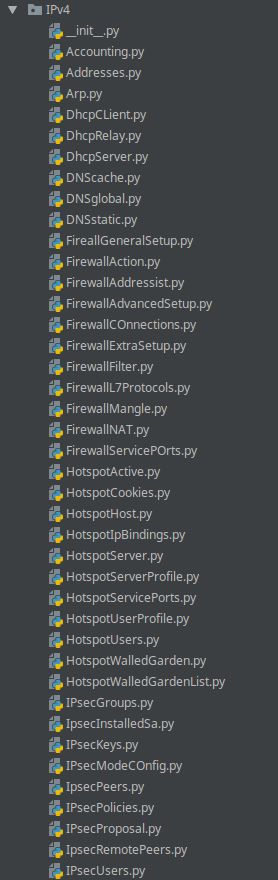
\includegraphics[scale=0.6]{../text/IP4.png}
\caption{Štruktúra časti zložky IPv4}
\label{fig:ipv4}
\end{figure}
\newpage
\subsection{Analýza vybraného súboru}
Vybraný súbor \textit{FirewallAddressist.py}popísaný UML diagramom na obrázku \ref{fig:addList} a obsah jeho metód je popísaný v tabuľke \ref{tab:addlist}.
\begin{table}[H]
\centering
\resizebox{\textwidth}{!}{%
\begin{tabular}{|c|c|c|c|}
\hline
Názov metódy & Vstup & Výstup & Vysvetlenie metódy \\ \hline
listAddressList & žiadny & slovník & Metóda vypíše zoznam address listov. \\ \hline
addAddressList & meno & slovník & Metóda pridá nový adress list. \\ \hline
removeList & meno & slovník & Metóda odstráni address list. \\ \hline
enableList & meno & slovník & Metóda zapne address list. \\ \hline
disableList & meno & slovník & Metóda vypne address list. \\ \hline
commentList & \begin{tabular}[c]{@{}c@{}}meno,\\ komentár\end{tabular} & slovník & Metóda nastaví komentár k záznamu v adress liste. \\ \hline
setName & \begin{tabular}[c]{@{}c@{}}číslo poradia záznamu,\\ meno\end{tabular} & slovník & Metóda zmení address list  v zázname. \\ \hline
setAddress & \begin{tabular}[c]{@{}c@{}}číslo poradia záznamu,\\ adresa\end{tabular} & slovník & Metóda zmení IP adresu položky. \\ \hline
setTimeout & \begin{tabular}[c]{@{}c@{}}číslo poradia záznamu,\\ timeout hodnota\end{tabular} & slovník & Metóda nastaví hodnotu timeoutu pre záznam v address liste. \\ \hline
\end{tabular}%
}
\caption{Obsah triedy FirewallAdressist}
\label{tab:addlist}
\end{table}
\begin{figure}[H]
\centering
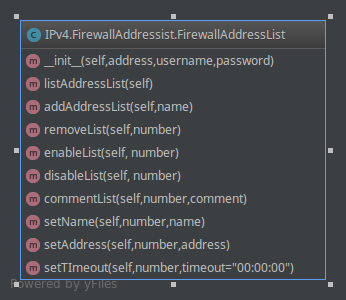
\includegraphics[scale=0.6]{../text/addList.png}
\caption{UML diagram triedy FirewallAddressist}
\label{fig:addList}
\end{figure}
\section{Zložka IPv6}
Podtstata zložky IPv6 je nastavenie IPv6 protokolu pozostavújecoho z DHCP pre IPv6, rozsahov adries, smerovania, firewallu a ďalších možností.
\subsection{Popis tried zložky}
Zložka obsahuje nastavenie funkcií prokolu IPv6 a zahrňuje:\begin{itemize}
\item \textbf{DHCPv6} - nastavenie protokolu DHCPv6 v triedach:\\
\textbf{DHCPRelay} - nastavenie DHCP Relay pre verziu IPv6\\
\textbf{DHCPServer} - nastavenie DHCP serveru\\
\textbf{DHCPv6Client} - nastavenie DHCPv6 klienta\\
\textbf{FirewallActions} - nastavenie firewall akcií - povolenie ,zahodenie, logovanie, ...\\
\textbf{FirewallAdvancedSetup} - nastavenie pokročilých vlastností firewallu napr. povolenie address listu, ...\\
\textbf{FirewallConnections} - Správa pripojení v o verzii IPv6\\
\textbf{FirewallExtraSetup} - Správa pokročilých nastavení napr. počet odoslaných paketov, ...\\
\textbf{FirewallFilter} -nastavenie filter pravidiel \\
\textbf{FirewallGeneralSetup} - nastavenie hlavných vlastností pravidlaa správa pravidiel\\
\textbf{FirewallMangle} - nastavenie QoSpre IPv6\\
\textbf{FirewallRaw} - nastavenie Raw (obdoba NAT)\\
\textbf{IPv6 AddressList}  - nastavenie address listu
\item \textbf{Addresses} - nastavenie a správa IPv6 adriesv triede \textbf{IPv6Addresses}
\item \textbf{Neighbors} - nastavenie a správa vyhľadávania pripojených zariadení v triede \textbf{IPv6NeighborDiscovery}
\item \textbf{Route} - správa smerovania v triede \textbf{IPv6Route}
\item \textbf{Settings} - správa nastavenia IPv6 na globálnej úrovni v triede \textbf{IPv6Settings}
\item \textbf{Neighbors} - správa pripojených zariadení v triede \textbf{Neighbors}
\item \textbf{Pool} - správa rozsahov adries v triede \textbf{Pool}
\end{itemize}
\begin{figure}[H]
\centering
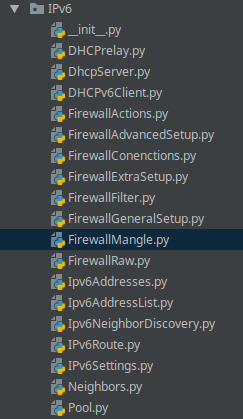
\includegraphics[scale=0.6]{../text/IPV6.png}
\caption{Zoznam súborov zložky IPv6}
\label{fig:ipv6}
\end{figure}
\subsection{Anylýza vybraného súboru}
Vybraný súbor \textit{FirewallManngle.py} je zobrazené UML diagramom triedy na obrázku \ref{fig:mangle} a obsah metód je zobrazený v tabuľke \ref{tab:ipv6mangle}.
\begin{table}[H]
\resizebox{\textwidth}{!}{%
\begin{tabular}{|c|c|c|c|}
\hline
Názov metódy & Vstup & Výstup & Vysvetlenie metódy \\ \hline
listRules & žiadny & slovník & Metóda vypíše zoznam pravidiel. \\ \hline
addRule & chain & slovník & Metóda pridá nové pravidlo. \\ \hline
removeRule & poradové číslo pravidla & slovník & Metóda odstráni pravidlo. \\ \hline
enableRule & poradové číslo pravidla & slovník & Metóda zapne pravidlo. \\ \hline
disableRule & poradové číslo pravidla & slovník & Metóda vypne pravidlo. \\ \hline
commentList & \begin{tabular}[c]{@{}c@{}}poradové číslo pravidla,\\ komentár\end{tabular} & slovník & Metóda nastaví komentár k pravidlu. \\ \hline
resetCounter & poradové číslo pravidla & slovník & Metóda zmaže počítadlo paketov a bytov pre konkrétne pravidlo. \\ \hline
resetAllCounters & žiadny & slovník & Metóda zmaže počítadlo všetkých pravidiel paketov a bytov. \\ \hline
\end{tabular}%
}
\caption{Tabuľka triedy FirewallMangle}
\label{tab:ipv6mangle}
\end{table}
\begin{figure}[H]
\centering
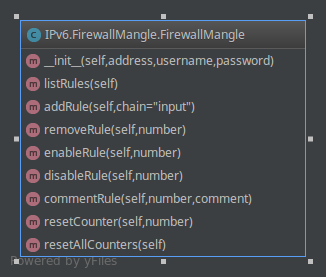
\includegraphics[scale=0.6]{../text/fwmangle.png}
\caption{UML diagram triedy FirewallMangle}
\label{fig:mangle}
\end{figure}
\section{Zložky KVM, log a makeSupportFile}
Obsahom zložiek je nastavenie virtuálneho mikrotiku, nastavenie logovania a vytvorenie súboru, ktorý je možné odslať na mikrotik podporu na analýzu. Celkový obsah je popísaný nižšie.
\subsection{Popis triedy zložky KVM}
Nastavenie virtuálnych mikrotikov alebo "mikrotiku v mikrotiku" je možné pomocou tzv. KVM. Zložka obsahuje triedy:\begin{itemize}
\item \textbf{KVM} - trieda na nastavenie virtualizácie na mikrotiku pomocou triedy \textbf{KVM}
\end{itemize}
\begin{figure}[H]
\centering
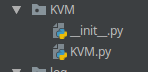
\includegraphics[scale=0.6]{../text/kvm.png}
\caption{Zoznam súborov zložky KVM}
\label{fig:mangle}
\end{figure}
Popis súboru \textit{KVM.py} je popísaný na obrázku \ref{fig:kvm}  a jeho obsah metód je popísaný v tabuľke \ref{tab:kvm}.
\begin{table}[H]
\resizebox{\textwidth}{!}{%
\begin{tabular}{|c|c|c|c|}
\hline
Názov metódy & Vstup & Výstup & Vysvetlenie metódy \\ \hline
listKVM & žiadny & slovník & Metóda zobrazí všetky virtuálne mikrotiky. \\ \hline
\end{tabular}%
}
\caption{Tabuľka metód triedy KVM}
\label{tab:kvm}
\end{table}
\begin{figure}[H]
\centering
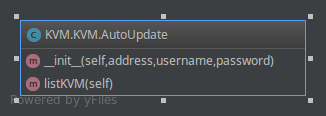
\includegraphics[scale=0.6]{../text/kvmfig.png}
\caption{UML diagram triedy KVM}
\label{fig:kvm}
\end{figure}
\subsection{Popis triedy zložky log}
Zložka log popisuje výpis systémového logu. Obsahuje triedy:\begin{itemize}
\item \textbf{log} - trieda log na výpis systémového logu
\end{itemize}
\begin{figure}[H]
\centering
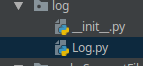
\includegraphics[scale=0.6]{../text/log.png}
\caption{Zoznam súborov zložky log}
\label{fig:log}
\end{figure}
Zoznam použitých metód je popísaný UML diagramom triedy na obrázku \ref{fig:logUML} a popísaný v tabuľke \ref{tab:log}.
\begin{table}[H]
\resizebox{\textwidth}{!}{%
\begin{tabular}{|c|c|c|c|}
\hline
Názov metódy & Vstup & Výstup & Vysvetlenie metódy \\ \hline
listLog & žiadny & slovník & Metóda zobrazí systémový log. \\ \hline
\end{tabular}%
}
\caption{Tabuľka metód triedy log}
\label{tab:log}
\end{table}
\begin{figure}[H]
\centering
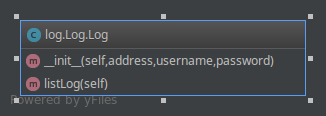
\includegraphics[scale=0.6]{../text/logUML.png}
\caption{UML diagram triedy log}
\label{fig:logUML}
\end{figure}
\subsection{Popis triedymakeSupportFile}
Zložka log obsahuje súbor makeSupportFile spološne striedou makeSupportFile, vytvorí a odošle súbor na podporu. Trieda makeSupport má na starosti vytvorenie súboru pre podporu na analýzu. Obsah súboru je popísanýv tabuľke \ref{tab:support} a UML diagramom triedy na obrázku \ref{fig:support}.
\begin{table}[]
\resizebox{\textwidth}{!}{%
\begin{tabular}{|c|c|c|c|}
\hline
Názov metódy & Vstup & Výstup & Vysvetlenie metódy \\ \hline
makeSupportFile & názov súboru & slovník & Metóda vytvorí súbor na podporu. \\ \hline
\end{tabular}%
}
\caption{Tabuľka metód triedy makeSupport}
\label{tab:support}
\end{table}
\begin{figure}[H]
\centering
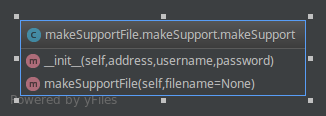
\includegraphics[scale=0.6]{../text/support.png}
\caption{UML diagram triedy makeSupport}
\label{fig:support}
\end{figure}
